\documentclass[spanish]{article}
\usepackage[spanish]{babel}
\usepackage{amsmath}
\usepackage{amssymb}
\usepackage[utf8]{inputenc}
\usepackage{vmargin}
\usepackage{graphicx}


\begin{document}
	\setpapersize{USletter}
	\setmarginsrb{30mm}{30mm}{30mm}{30mm}{0pt}{0mm}{0pt}{0mm}
	
	\begin{center}
	{\Large Análisis de Algoritmos, Sem: 2018-1, 3CV2 Práctica 1, 24-08-2017}\\
{\huge {\bf Práctica 1: Determinación experimental de
la complejidad de un algoritmo}} \\
{\large {\bf Salgado Alarcon Genaro, Padilla Calderon Jose Manuel}\\
Escuela Superior de Cómputo \\
Instituto Politécnico Nacional}\\
isomaelking@gmail.com, genaro\_yen13@hotmail.com\\	
	\end{center}
	\bigskip
	
	\bigskip
	
	\bigskip
	
	{\LARGE {\bf Primero}}\\
En este trabajo vamos a analizar, por medio de  la
 experimentación, la complejidad de un  algoritmo dado,  proponiendo  una 
función g(n) tal que Suma $\in$ O(g(n)) y g(n) sea mínima, en el sentido 
de que si Suma $\in$ O(h(n)), entonces g(n) $\in$ O(h(n)). 
Obserando como se comporta, se compará el  comportamiento entre 
el tiempo de ejecución y un número de veces que se ejecuta la llamada a la función.
\bigskip


	{\Large {\bf Palabras Clave}}\\
	\begin{itemize}
		\item Algoritmo
		\item Funcion
		\item Experimentacion
		\item Eficiencia
	\end{itemize}
	\bigskip
	
	\section{Introducci\'on}
	Todos los días nos enfrentamos a problemas en los que usamos un algoritmo para resolverlos, es importante observar que quiza no estemos empleando la mejor solucion a estos problemas. 
	Tanto en la vida cotidiana como en la industria se usan algoritmos que nos ayudan a optimizar nuestro trabajo, trabajo que significa esfuerzo y dinero en algunas ocaciones, por lo tanto
	es importante el estudio de estos algoritmos, en este trabajo, por medio de la experimentacion vamos a analizar que tan eficiente y complejo puede ser un algoritmo, para así poder encontrar una mejor soluciona este
	lo que puede significar ahorrar tanto tiempo, como esfuerzo y quiza dinero.
	\bigskip
\newpage
	\section{Conceptos B\'asicos}
	Para la correcta comprension de este trabajo, es necesario definir algunos terminos tales como $\theta$, O y $\Omega$.\\
	 $\theta$(n):\\
		Sea g(n) una función. Se define  $\theta$ (g(n)) como:\\
		
		 	$\theta$(g(n)) = $\{ f(n) \quad | \quad \exists c1,c2>0 \quad \& \quad n_{0}>0 \quad \mid \quad \forall n>=n_{0} \quad 0<= c1g(n) <= f(n) <= c2g(n) \}$
	\bigskip		 	
		 	
	O(n):\\
		Sea  g(n)  una función, O(n) se define como:\\
		
			\hspace{1cm}O(n)=$\{f(n) \quad | \quad \exists c >0 \quad \& \quad n_{0}>0 \quad | \quad f(n) <= Cg(n) \quad \forall  n>= n_{0} \}$
	\bigskip
	
	$\Omega$(n):\\
	Sea  g(n)  una función. Se define $\Omega$ (g(n)) como:\\

		\hspace{1cm}$\Omega$(g(n)) =$\{f(n) \quad | \quad \exists c >0 \quad \& \quad n_{0}>0 \quad \mid \quad  0<= cg(n)<= f(n) \quad \forall n>= n_{0} \}$
	\bigskip

	Se muestra experimentalmente el tiempo computacional de dos algoritmos y un tercero de manera teórica, 
	el primer algoritmo de desarrollo experimental consiste en sumar dos números enteros en notación binariaconsiderando que: 
	Dos arreglos unidimensionales A de tamaño n y B de tamaño m con k = $\log_{2}(n)$ y t = $\log{2}(m)$ almacenarán los números a sumar. 
	La suma se almacenará en un arreglo C. El propósito es obtener el tiempo que se tarda en realizar dicha operación con un tamaño r que se le asigna al arreglo.
	
	\begin{center}
		%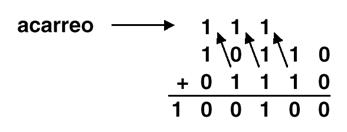
\includegraphics{binario.jpg}\\
		Figura 1
	\end{center}
	
La Figura 1 ejemplifica la operación que se realiza en una suma binaria, se toma las siguientes cuestiones:\\
\begin{itemize}
	\item 0+0=0
\item 0+1=1
\item 1+0=1
\item 1+1=0 y se lleva uno
\end{itemize}

El segundo algoritmo experimental  consiste en  implementar el algoritmo de Euclides para encontrar el mcd de dos números enteros positivos m y n. 
El propósito al igual que el anterior algoritmo es obtener el tiempo de ejecución cuando se mande a llamar la función de Euclides, 
pero con la condición que los números a los que se obtendrá el m.c.d serán los que se obtienen de la serie de Fibonacci, 
los cuales se obtienen de la suma de los dos números que le preceden 
1 ,1,2,3,5,8,13,21,34 ,etc, se toma por ejemplo el 8,13 y se llama a la función Euclides(8,13) el cual dará como resultado un número “n” tal que 8\%n=0 y 13\%n=0.

Para el algoritmo teórico se encontrará la complejidad de un programa de ordenamiento.
	
\newpage	
\section{Experimentaci\'on y Resultados}
	\subsection{Suma Binaria}
	{\large{\bf-Pseudoc\'odigo Suma Binaria}}\\
	Suma (A,B,n[1,...,17],c)\\
Entrada: i[1,..., 17]\\
Salida: Tiempo computacional de n[1,...,17]\\
1. for i $\leftarrow$ 1 to i $\leftarrow$ 17 do\\
2.		\hspace{0.7cm}n $\leftarrow$ potencia(2,i)\\
3.      \hspace{0.7cm}suma(A,B,n,c)\\
4. 		\hspace{0.7cm}print(c)
\bigskip

	{\large{\bf-Mostrar gráficas para la función Suma que muestre tiempo vs r con r = m = n (considere diversos valores de r).}}\\
	\begin{center}
				%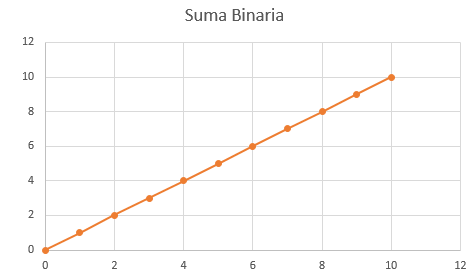
\includegraphics{g1.PNG}\\
		Figura 2\\
	\end{center}
	
	La tabla p[ara esta grafica es:\\
	\begin{center}
		%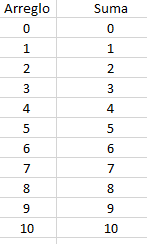
\includegraphics{t1}\\
		Figura 3\\
	\end{center}

	
	
	{\large{\bf -Proponer una función g(n) tal que S $\in$ O(g(n)) y g(n) sea mínima, en el sentido de que si S $\in$  O(h(n)), entonces g(n) $\in$  O(h(n)).}}\\
	Por los resultados obtenidos en la gráfica proponemos que la complejidad del algoritmo S es de tipo lineal, y se propone la función O(n).
	\bigskip
	
	{\large {\bf -Conclusiones}}\\
	
{\bf Genaro Salgado Alarcon}:.\\A mi perspectiva el ejercicio con los temas vistos en clase fue algo sencillo de analizar, porque si, cuando lo leímos por primera vez en verdad se complico un poco el entenderlo, pero, si tienes los apuntes completos y los consultas mientras desarrollas el ejercicio, se hará mas sencillo de entender, al igual que con la suma binaria, tuvimos que consultar los apuntes para entenderlo por completo\\
{\bf Padilla Calderon Jose Manuel}:.\\La suma fue un poco complicado complicada, al menos un poco mas que el de Euler si, tanto en el nivel de análisis como en programación, porque entender exactamente lo que se solicitaba era algo que nos preocupaba para cumplir completamente con la practica, nuestro primer problema fue que terminábamos el script y nos dábamos cuenta que teníamos que hacer otras cosas, entonces, obviamente teníamos que completar el script.
\\
	
	
	\bigskip
	
	\bigskip
	\newpage
	\subsection{Euclides}
	{\large{\bf1.- Pseudoc\'odigo Algoritmo de Euclides}}\\
	Euclides (A,B,c]\\
Entrada: fibonacci(n),fibonacci(n-1) con $1<=n<50$\\
Salida: Tiempo computacional de $1<=n<50$\\
1.  for i $\leftarrow$ 1 to i $\leftarrow$ 79 do\\
2.      \hspace{0.7cm}a $\leftarrow$ fibonacci(i)\\
3.      \hspace{0.7cm}b $\leftarrow$ fibonacci(i+1)\\
4.      \hspace{0.7cm}e $\leftarrow$ euclides(b,a,c)\\
5.	   \hspace{0.7cm}print(c)\\

\bigskip

	{\large{\bf -Mostrar gráficas para la función Euclides que muestre tiempo vs diferentes valores de m y n.}}\\
	Para valores del fibonacci de 1 a 79
	\begin{center}
			%\includegraphics{tabla21}\\	
	%\includegraphics{tabal22}\\

		Figura 5\\
	\end{center}

	La gráfica es:\\
	\begin{center}
		%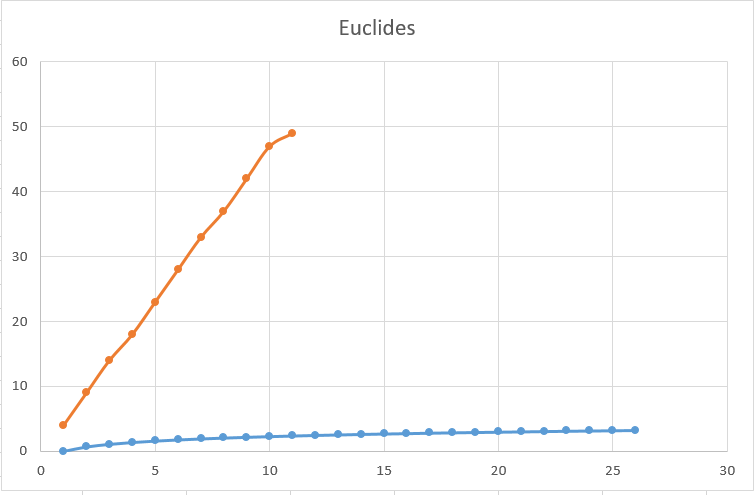
\includegraphics{euclides}\\
		Figura 6\\
	\end{center}

	{\large{\bf -Proponer una función g(n) tal que Euclides $\in$ O(g(n)) y g(n) sea mínima, en el sentido de que si Euclides $\in$  O(h(n)), entonces g(n) $\in$  O(h(n)).}}\\
	Por los resultados obtenidos en la última gráfica proponemos que la complejidad del algoritmo Euclides es de tipo logarítmica y propones la función O($\log_{2}(n)$) ya que O($\log_{2}(n)$) pasa ser cota superior cumpliendo así la definición de O($\log_{2}(n)$).
	\bigskip
	
	{\large {\bf -Conclusiones}}\\
	{\bf Genaro Salgado Alarcon}:.
	El ejercicio de Euler se nos complico en el inciso de Fibonacci porque estábamos programando todo para poder compararlo, pero nos dimos cuenta que teníamos que analizar lo que nos pedía que era entender el mcd y su relación con la serie de fibonacci mas no el código, después de entender esto se facilito el análisis teórico, ya con esto pudismos completar el ejercicio. \\
{\bf Padilla Calderon Jose Manuel}:.\\Este ejercicio fue un poco mas sencillo al momento de programar ya que era un problema sencillo, peor en el análisis nos fue un poco mas complicado resolverlo ya que su curva fue logarítmica según los resultados que obtuvimos, no fue tan sencillo como en la suma donde todo era lineal, es importante mencionar que el pseudocodigo que vimos en el pdf de la practica nos fue de gran ayuda para empezar a programar y entender.
\\

	\newpage
	\section{Conclusi\'on General}
	Esta primer practica como ya lo hemos explicado a lo largo del desarrollo de esta, nos ha presentado una nueva visión no solo de 	los algoritmos sino de la programación en general, es cierto que hoy en día existen muchísimas maneras para hacer un correcto programa, tanto documentación como otras, que radican desde el logaritmo mismo, esta materia nos ha abierto el panorama a los primeros métodos de análisis de algoritmos, para así, más tarde poder decir si nuestro algoritmo es válido o no, la practica nos presentó un tema de digitales, el cual nos fue más fácil de lo normal ya que estos temas no nos son ajenos,  el mayor problema fue el de entender las características del reporte para que cumpliera con los rubros de la entrega.
	\newpage
	\section{Anexos}
	
	{\Large{\bf Select-Sort}}\\
	Select-Sort(A[0...n-1]) \hspace{2.9cm}Costo \hspace{1.7cm} \#Pasos \\
	1.-	\hspace{0.7cm}for j $\leftarrow$ 0 to n-2 do \hspace{2.3cm} C1 \hspace{2.0cm} n\\
	2.-		\hspace{1.4cm}k $\leftarrow$ j\hspace{3.8cm} C2 \hspace{2.0cm} n-1\\
	3.-		\hspace{1.4cm}for i $\leftarrow$ j+1 to n-1 do \hspace{1.3cm} C3 \hspace{2.0cm}$\sum_{i=0}^{n-1}t_{i}$\\
	4.-			\hspace{2.1cm}if A[i] $<$ A[k] then \hspace{1.1cm} C4 \hspace{2.0cm}$\sum_{i=0}^{n-1}(t_{i}-1)$\\
	5.-				\hspace{2.8cm}k $\leftarrow$ i \hspace{2.4cm} C5 \hspace{2.0cm}$\sum_{i=0}^{n-1}R_{i}$\\
	6.-	\hspace{1.4cm} intercambia(A[j],A[k]) \hspace{1.2cm} C6 \hspace{2.0cm}n-1\\
	\bigskip
	
	\bigskip
	
	El peor de los casos se presenta cuando el arreglo esta ordenado en forma decreciente por lo  que:\\ 
	$t_{i} = n-i$ y\\
	$R_{i} = n-i-1 = t_{i}-1$\\
	\bigskip
	
	Por lo tanto tenemos que:\\
	T(n) = C1n + C2(n-1) + C3($\sum_{i=0}^{n-1}(n-i)$) + C4($\sum_{i=0}^{n-1}(n-i-1)$) + C5($\sum_{i=0}^{n-1}(n-i-1)$) + C6(n-1)
	\bigskip
	
	T(n) = C1n + C2n -C2 + C3($\sum_{i=0}^{n-1}n$) - C3($\sum_{i=0}^{n-1}i$) + C4($\sum_{i=0}^{n-1}n$) - C4($\sum_{i=0}^{n-1}i$) - C4($\sum_{i=0}^{n-1}1$) + C5($\sum_{i=0}^{n-1}n$) -C5 ($\sum_{i=0}^{n-1}i$) - C5($\sum_{i=0}^{n-1}1$) + C6n -C6
	\bigskip
	
	T(n) = (C1+C2+C6)n + (C3+C4+C5)($n^{2}$) - (C3+C4+C5)($\sum_{i=1}^{n}(i-1)$) - (C4+C5)n -(C2+C6)
	\bigskip
	
	T(n) = (C3+C4+C5)$n^{2}$ -(C3+C4+C5)($\dfrac{n(n+1)}{2}$ - n) +(C1+C2-C4-C5+C6)n - (C2+C6)
	\bigskip
	
	T(n) = ($\dfrac{C3+C4+C5}{2}$)$n^{2}$	+ (C1+C2+C3+C6)n - (C2+C6)
	\bigskip
	
	$\therefore$
	$ T(n) \quad \in \quad O(n^{2})$
	\bigskip	
	
	\section{Bibliografía}
	\begin{itemize}
		\item Brassard, G. (1997). Fundamentos de Algoritmia. España: Ed. Prentice Hall. ISBN 		848966000X
		\item Harel, D. (2004). Algorithmics: The spirit of Computing (3rd. Ed). Estados Unidos de América: Addison
Wesley. ISBN-13: 978-0321117847
	\end{itemize}
	
\end{document}